\documentclass[10pt]{exam}
\usepackage[phy]{template-for-exam}
\usepackage{pgfplots}
\pgfplotsset{
    compat=1.18,
    reg/.append style={
        xmin =-4.5,
        xmax =4.5,
        ymin =-4.5,
        ymax = 4.5,
        axis lines = center,
        xtick = {-4,...,4},
        ytick = {-4,...,4},
        height = 6cm,
        width = 6cm,
        grid = major,
        grid style = {thick, dotted},
        tick label style = {font=\small}
      },
    myplot/.append style={
      smooth,domain=-4:4,samples=50,thick
    },
    wave/.style={
      width=5cm,
      height=5mm,
      scale only axis,
      ultra thick,
      xmin=0,
      xmax=10,
      hide axis
    }
  }

\title{Waves \#2}
\author{Rohrbach}
\date{\today}

\begin{document}
\maketitle

\begin{questions}

\question
  The wave below is traveling at 20~m/s.  All measurements are in meters.

  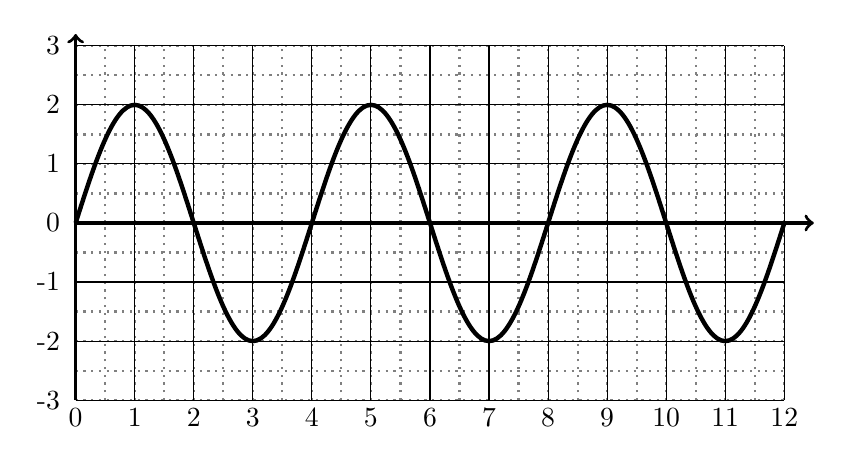
\begin{tikzpicture}[scale=0.75]
    \def\wl{4}
    \def\amp{2}
    \def\ymax{3}
    \def\xmax{12}
    \draw[dotted,thick,gray] 
      (0,-\ymax*1cm) grid[step=0.5cm] (\xmax*1cm,\ymax*1cm);
    \draw 
      (0,-\ymax*1cm) grid[step=1cm] (\xmax*1cm,\ymax*1cm);
    \foreach \x in {0,...,\xmax}{
      \draw (\x*1cm,-\ymax*1cm) ++(0,-.3cm) node {\x};
    }
    \foreach \y in {-\ymax,...,\ymax}{
      \node[anchor=east] at (-0.1cm,\y*1cm) {\y};
    }
    \draw[very thick,->] 
      (0,0) -- (\xmax*1cm,0) -- ++(0.5cm,0);
    \draw[very thick,->] 
      (0,-\ymax*1cm) -- (0,\ymax*1cm) -- ++(0,0.2cm);

    \draw[ultra thick] (0,0) 
      sin (0.25*\wl, \amp) cos (0.5*\wl, 0) 
      sin (0.75*\wl,-\amp) cos (    \wl, 0)
      sin (1.25*\wl, \amp) cos (1.5*\wl, 0)
      sin (1.75*\wl,-\amp) cos (2.0*\wl, 0)
      sin (2.25*\wl, \amp) cos (2.5*\wl, 0)
      sin (2.75*\wl,-\amp) cos (3.0*\wl, 0);
  \end{tikzpicture}

  \begin{parts}
    \part 
      What kind of wave is this? \vs
    \part 
      What is its amplitude? \vs
    \part 
      What is the wavelength? \vs
    \part 
      What is the frequency? \vs

  \end{parts}

  
\question
  These two waves have the same velocity.  Which one has a higher frequency?  How can you tell?
  
  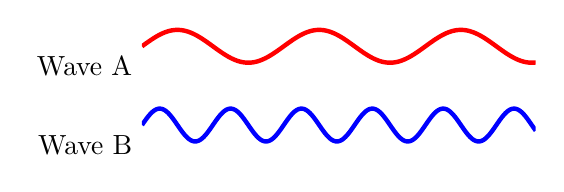
\begin{tikzpicture}
    \begin{scope}
      \node[anchor=east] at (0,0) {Wave A};
      \begin{axis}[red,wave] 
        \addplot[domain=0:10,samples=900]{sin(100*x)};
      \end{axis}
    \end{scope}

    \begin{scope}[shift={(0,-1)}]
      \node[anchor=east] at (0,0) {Wave B};
      \begin{axis}[blue,wave] 
        \addplot[domain=0:10,samples=900]{sin(200*x)};
      \end{axis}
    \end{scope}
  \end{tikzpicture}
  \vspace{2em}


\question
  Draw a wave with an amplitude of 1.5~m and a wavelength of 6~m.

    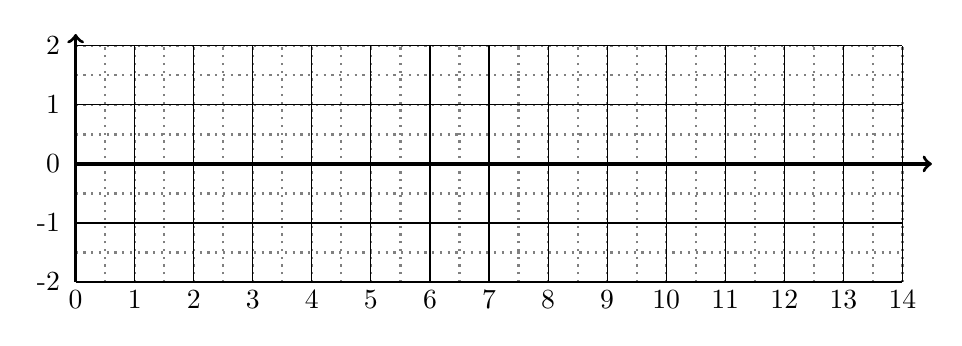
\begin{tikzpicture}[scale=0.75]
      \def\ymax{2}
      \def\xmax{14}
      \draw[dotted,thick,gray] 
        (0,-\ymax*1cm) grid[step=0.5cm] (\xmax*1cm,\ymax*1cm);
      \draw 
        (0,-\ymax*1cm) grid[step=1cm] (\xmax*1cm,\ymax*1cm);
      \foreach \x in {0,...,\xmax}{
        \draw (\x*1cm,-\ymax*1cm) ++(0,-.3cm) node {\x};
      }
      \foreach \y in {-\ymax,...,\ymax}{
        \node[anchor=east] at (-0.1cm,\y*1cm) {\y};
      }
      \draw[very thick,->] 
        (0,0) -- (\xmax*1cm,0) -- ++(0.5cm,0);
      \draw[very thick,->] 
        (0,-\ymax*1cm) -- (0,\ymax*1cm) -- ++(0,0.2cm);
    \end{tikzpicture}
  
  \end{questions}
    
\end{document}